\tableofcontents
\newpage

\section{Цель работы}
По выданному преподавателем варианту восстановить текст заданного варианта программы, определить предназначение и составить описание программы, определить область представления и область допустимых значений исходных данных и результата, выполнить трассировку программы.
\begin{figure}[H]
\centering
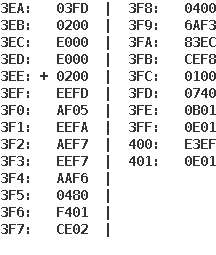
\includegraphics[scale=0.6]{task}
\label{pic:task}
\end{figure}
              
\section{Текст программы}
\noindent
\begin{center}
\begin{tabular}{|c|c|c|l|}
\hline
\multicolumn{1}{|c}{\makecell{\textbf{Адрес}\\\textbf{ячейки}}}
&\multicolumn{1}{|c|}{\makecell{\textbf{Содержимое}\\\textbf{ячейки}}}
&\multicolumn{1}{|c|}{\makecell{\textbf{Мнемоника}}}
&\multicolumn{1}{c|}{\makecell{\textbf{Комментарии}}}\\
\hline	

\hline	

3E8 & 3FB & --- & Адрес начала массива \\

3E9 &  & --- & Ячейка для хранения адреса обрабатываемого \\
& & & элемента массива \\

3EA &  & --- & Ячейка для хранения количества необработанных \\
& & & элементов массива \\

3EB &  & --- & \\

\hline
\hline
3EC & 0200 & CLA & Очистка аккумулятора \\

3ED &  &  & \\

3EE &  &  & \\

3EF &  &  & \\

3F0 &  &  & \\

3F1 &  &  & \\

3F2 &  &  & \\

3F3 &  &  & \\

3F4 &  &  & \\

3F5 &  &  & \\

3F6 &  &  & \\

3F7 &  &  & \\

3F8 &  &  & \\

3F9 &  &  & \\

3FA & 0100 & HLT & Остановка \\

\hline
\hline
3FB &  & --- & \\

3FC &  & --- & \\

3FD &  & --- & Элементы массива \\

3FE &  & --- & \\

3FF &  & --- & \\

\hline
\end{tabular}
\end{center}

\section{Описание программы}
\subsection{Назначение программы и реализуемая ею функция (формула)}
\subsection*{Назначение программы}
\noindent

\subsection*{Реализуемая функция (формула)}
\noindent $=$

\subsection{Область представления и область допустимых значений исходных данных и результата}

\subsection*{Область представления}
\noindent
Исходные данные: \\
Aдрес начала массива: 11-разрядные беззнаковые числа, с фиксированной запятой.\\
Диапазон значений: $0\ldots2^{11}-1$ \\
Элементы массива: 16-разрядные знаковые числа, фиксированной запятой.\\
Диапазон значений:  $-2^{15}\ldots2^{15}-1$ \\\\
Результат: \\
Счетчик нечетных элементов: 16-разрядное беззнаковое число, фиксированной запятой.\\
Диапазон значений:  $0\ldots2^{15}-1$

\subsection*{Область допустимых значений}
\noindent Исходные данные: \\
Aдрес начала массива: [000, ***] $\cup$ [***, ***] \\
Элементы массива: $-2^{15}\ldots2^{15}-1$\\\\
Результат: $0\ldots*$

\subsection{Расположение в памяти ЭВМ программы, исходных данных и результатов}
\noindent Программа: ***--*** \\
Исходные данные: \\
Aдрес начала массива: *** (Z $=$ Содержимое ячейки 3EA) \\
Элементы массива: ***--*** (Z--(Z$+$4), элемент массива: $X_{i}$) \\
Вспомогательные ячейки: ***, *** \\
Результат: *** (Y $=$ Содержимое ячейки ***)

\subsection{Адреса первой и последней выполняемой команд программы}
\noindent Адрес первой выполняемой команды : *** \\
Адрес последней выполняемой команды: ***

\section{Таблица трассировки}
\begin{flushleft}
\begin{tabular}{|c|c|c|c|c|c|c|c|c|c|c|c|}
\hline
\multicolumn{2}{|c}{\makecell{\textbf{Выполняемая}\\\textbf{команда}}}
  &\multicolumn{8}{|c|}{\textbf{Содержимое регистров после выполнения команды}}
  &\multicolumn{2}{c|}{\makecell{\textbf{Ячейка, }\\\textbf{содержимое}\\\textbf{которой}\\\textbf{изменилось}}}\\
\hline
Адрес & Код & IP & CR & AR & DR & SP & BR & AC & NZVC & Адрес & Новый код\\
&  &  &  &  &  & 000 &  &  &  & --- & ---	 \\\hline

&  &  &  &  &  & 000 &  &  &  & --- & ---	 \\\hline

&  &  &  &  &  & 000 &  &  &  & --- & ---	 \\\hline

&  &  &  &  &  & 000 &  &  &  & --- & ---	 \\\hline

&  &  &  &  &  & 000 &  &  &  & --- & ---	 \\\hline

&  &  &  &  &  & 000 &  &  &  & --- & ---	 \\\hline

&  &  &  &  &  & 000 &  &  &  & --- & ---	 \\\hline

&  &  &  &  &  & 000 &  &  &  & --- & ---	 \\\hline

&  &  &  &  &  & 000 &  &  &  & --- & ---	 \\\hline

&  &  &  &  &  & 000 &  &  &  & --- & ---	 \\\hline

&  &  &  &  &  & 000 &  &  &  & --- & ---	 \\\hline

&  &  &  &  &  & 000 &  &  &  & --- & ---	 \\\hline

&  &  &  &  &  & 000 &  &  &  & --- & ---	 \\\hline

&  &  &  &  &  & 000 &  &  &  & --- & ---	 \\\hline

&  &  &  &  &  & 000 &  &  &  & --- & ---	 \\\hline

&  &  &  &  &  & 000 &  &  &  & --- & ---	 \\\hline

&  &  &  &  &  & 000 &  &  &  & --- & ---	 \\\hline

&  &  &  &  &  & 000 &  &  &  & --- & ---	 \\\hline

&  &  &  &  &  & 000 &  &  &  & --- & ---	 \\\hline

&  &  &  &  &  & 000 &  &  &  & --- & ---	 \\\hline

&  &  &  &  &  & 000 &  &  &  & --- & ---	 \\\hline

&  &  &  &  &  & 000 &  &  &  & --- & ---	 \\\hline

&  &  &  &  &  & 000 &  &  &  & --- & ---	 \\\hline

&  &  &  &  &  & 000 &  &  &  & --- & ---	 \\\hline

&  &  &  &  &  & 000 &  &  &  & --- & ---	 \\\hline

&  &  &  &  &  & 000 &  &  &  & --- & ---	 \\\hline

&  &  &  &  &  & 000 &  &  &  & --- & ---	 \\\hline

&  &  &  &  &  & 000 &  &  &  & --- & ---	 \\\hline

&  &  &  &  &  & 000 &  &  &  & --- & ---	 \\\hline

&  &  &  &  &  & 000 &  &  &  & --- & ---	 \\\hline

&  &  &  &  &  & 000 &  &  &  & --- & ---	 \\\hline

&  &  &  &  &  & 000 &  &  &  & --- & ---	 \\\hline

&  &  &  &  &  & 000 &  &  &  & --- & ---	 \\\hline

&  &  &  &  &  & 000 &  &  &  & --- & ---	 \\\hline

&  &  &  &  &  & 000 &  &  &  & --- & ---	 \\\hline

&  &  &  &  &  & 000 &  &  &  & --- & ---	 \\\hline

&  &  &  &  &  & 000 &  &  &  & --- & ---	 \\\hline

&  &  &  &  &  & 000 &  &  &  & --- & ---	 \\\hline

&  &  &  &  &  & 000 &  &  &  & --- & ---	 \\\hline

&  &  &  &  &  & 000 &  &  &  & --- & ---	 \\\hline
\end{tabular}
\end{flushleft}

\section{Диапазон всех ячеек памяти, где может размещаться массив исходных данных}
Диапазон: [***, ***] $\cup$ [***, ***]

\section{Вывод}
В ходе выполнения данной лабораторной работы я познакомился с режимами адресации БЭВМ и новыми для меня командами - ветвления, сравнения, командой LOOP. На практике разобрался с циклом выборки адреса для разных режимов адресации.